\chapter{Test des Systems}
\label{chapter:testing}

	\todo{Eventuell Anforderungen, die ominös angesprochen werden, direkt referenzieren.}
	Das Testen des Softwaresystem wurde in drei Aufgabenbereiche unterteilt.
	Zuerst wurde das Frontend durchgängig getestet.
	Anschließend wurde das Backend überprüft.
	Letztendlich wurde der Algorithmus und die Auswirkung diesen auf Richtigkeit untersucht.\newline
	
	Es gibt außerdem einige Verweise auf Testskripts, welche mit Laravel Dusk ausgeführt werden können.
	Um diese auf einer lokal laufenden Kopie auszuführen, kann das Skript \glqq runTests.sh\grqq~in einem Terminal genutzt werden.\newline
	
	\section{Frontend}
		Um das Frontend ordnungsgemäß zu testen, wurden verschiedene Testobjekte betrachtet.
		Im Folgenden werden diese erläutert.
		
		\subsection{Homepage}
			Zum Testen der Homepage steht das Testskript \textit{HomepageTest} zur Verfügung.
			Das Testskript überprüft dabei nur den Header der Website, da dies genügt.
			Dies bedeutet, dass sowohl die Textfelder des Headers, also \glqq Start\grqq, \glqq Kursübersicht\grqq, \glqq Meine Präferenzliste\grqq, und \glqq Ergebnis sehen\grqq, als auch die Reihenfolge derer verifiziert wird.
			Gleichermaßen werden auch die Buttons im Header, \glqq Anmelden\grqq~und \glqq Registrieren\grqq, überprüft.\newline
		
		\subsection{Registrierung}
			Der Testfall \textit{RegisterTest} verifiziert, dass ein Nutzer sich ordnungsgemäß registrieren kann und sich anschließend mit diesen Daten anmelden kann.
			Dafür ruft der automatisierte Nutzer die Homepage auf und gelangt über den \glqq Registrieren\grqq -Button zum Registrierungsformular.
			Dort gibt er seine Daten ein.
			Anschließend ruft der User die Login-Seite über den \glqq Anmelden\grqq -Button auf und meldet sich mit den Daten aus der Registrierung an. \newline
			Ein erfolgreicher Login wird durch die Abwesenheit des \glqq Anmelden\grqq -Buttons sicher gestellt.
			Am Ende des Tests wird der neu registrierte Nutzer gelöscht.\newline
		
		\subsection{Login}
			Der daran anschließende Testfall ist \textit{LoginTest}.
			Dieser verifiziert, dass ein bereits registrierter Nutzer sich anmelden kann.
			Dafür wird zuerst ein Benutzer in der Datenbank kreiert.
			Anschließend wird die Login-Seite geöffnet und die Daten des kreierten Nutzers eingegeben.
			Der erfolgreiche Login wird durch die Abwesenheit des \glqq Anmelden\grqq -Buttons sicher gestellt.
			Am Ende des Tests wird der kreierte Nutzer aus der Datenbank gelöscht.\newline
		
		\subsection{Kursübersicht}
			Die Kursübersicht wurde manuell getestet.
			Dafür wurden zuerst Kurse im Backend erstellt.
			Anschließen wurden sie im Frontend unter dem Menüpunkt \glqq Kursübersicht\grqq~auf Richtigkeit überprüft.
			Hierbei ist es wichtig, dass in dem Einführungstext der Übersicht das korrekte Jahr steht.
			Daraufhin wurde die Vorschau der Kurse kontrolliert.
			Dafür wurde sichergestellt, dass der Kurstitel, die Kurzbeschreibung, Ort, Zeit und ein Ausschnitt der ausführlichen Beschreibung dargestellt ist.
			Weiterhin musste jede Vorschau einen \glqq Details\grqq -Button beinhalten, der zur kompletten Kursbeschreibung führt.
			Diese musste und hat den Anforderungen entsprochen.\newline
		
		\subsection{Meine Präferenzliste}
			Anschließend wurde der Menüpunkt \glqq Meine Präferenzliste\grqq~manuell überprüft.
			Hier müssen alle Kurse sichtbar sein, die in diesem Semester gewählt werden können.
			Insbesondere ist es wichtig, dass jeder Kurs einzeln per \textit{Drag and Drop} verschoben werden kann.
			Nachdem Kurse anders platziert wurden, musste die Liste gespeichert werden.\newline
			Bei einem erneuten Aufruf des Menüpunktes muss die editierte Liste in der zuletzt verschobenen Reihenfolge angezeigt werden.
			Dies wurde verifiziert, indem die Cookies und der Cache geleert wurden und anschließend die Seite neu aufgerufen wurde.\newline
		
		\subsection{Ergebnis sehen}
			Der Menüpunkt \glqq Ergebnis sehen\grqq~ wurde manuell überprüft.
			Es wurde sicher gestellt, dass alle Nutzer, die eine Präferenzliste abgeschickt haben, in der Übersicht auftauchen.\newline
		
	\section{Backend}
	
		Für das Backend war es wichtig. zu verifizieren, dass sowohl Lehrstühle, Module, und Kurse, als auch neue Dozenten und Administratoren erstellt werden können.
			
		\subsection{Anlegen neuer Dozenten und Administratoren}
		
			Das Anlegen neuer Dozenten und Administratoren erfolgt im Backend unter dem Menüpunkt "Einstellungen" und anschließend unter \glqq Administratoren\grqq .
			Jeder Benutzer des Backends ist Administrator.
			Die Rechte eines Backend-Users wird über ein Rollen-System verwaltet.\newline
			Unabhängig des Rollen-Systems wurde verifiziert, dass ein Einloggen im Backend einen bereits registrierten Nutzer benötigt und die Daten zum Anmelden korrekt sein müssen.\newline
			Für jede Rolle, das heißt Dozent und Administrator, wurde weiterhin getestet, dass sie die konfigurierten Rechte nur besitzen.\newline
			Zuletzt wurde verifiziert, dass die Rechte der Dozenten und Administratoren den Anforderungen genügen.
			
		\subsection{Erstellen von Lehrstühlen, Modulen und Kurse}
			
			Das Erstellen von Lehrstühlen, Modulen und Kurse erfolgt im Backend unter dem Menüpunkt \glqq Verwalten\grqq .\newline
			Ein Testskript für das Erstellen von Lehrstühlen wurde unter dem Namen \glqq CreateChair\grqq~bereit gestellt.
			Da das Erstellen von Module und Kurse denselben Prinzipien folgt, wurden hierfür keine weiteren Skripte erstellt.
			Bei diesen wurde daher manuell statt automatisiert sicher gestellt, dass die nach den Anforderungen benötigten Felder existieren und die Pflichtfelder ausgefüllt werden müssen.\newline
			Weiterhin wurde verifiziert, dass Änderungen an bereits erstellten Kursen, etc. wirksam sind.
			Das heißt, ändert ein Dozent seinen Kurs, muss und ist diese Änderung sofort im Frontend sichtbar ist.
	
	\section{Algorithmus}
	
		Um den Algorithmus zu testen, mussten Daten generiert und in die Datenbank importiert werden.
		Dafür wurde zuerst ein R-Skript geschrieben, welches eine Präferenzenmatrix aus beliebig vielen Studenten und Kursen generiert.
		Mithilfe eines weiteren Skripts wurde dieses Datenset in die Datenbank des Servers importiert.
		Anschließend konnte die Verteilung im Backend ausgelöst werden.\newline
		
		Zur Evaluierung des Ergebnisses wurden künstliche Daten durch das R-Skript erzeugt und verwendet.
		Für die künstlichen Daten wurde einmal eine Gleichverteilung zur Erzeugung der Präferenzenmatrix genutzt, und zusätzlich eine Normalverteilung.
		Daraus ergaben sich dann zwei Dateien, die in die Datenbank importiert werden konnte.\newline
		Weiterhin wurden die Präferenzen des Empiriepraktikums aus dem Wintersemester 2017/2018 bereit gestellt.
		Dadurch konnte der neue Algorithmus direkt mit dem alten Verteilungsalgorithmus verglichen werden.
		Dies hatte zusätzlich zur Folge, dass das Erfüllen des Akzeptanzkriterium für den neuen Algorithmus klar definiert werden konnte.
		
		\subsection{Gleichverteilung}
	
			\begin{figure}
				\centering
				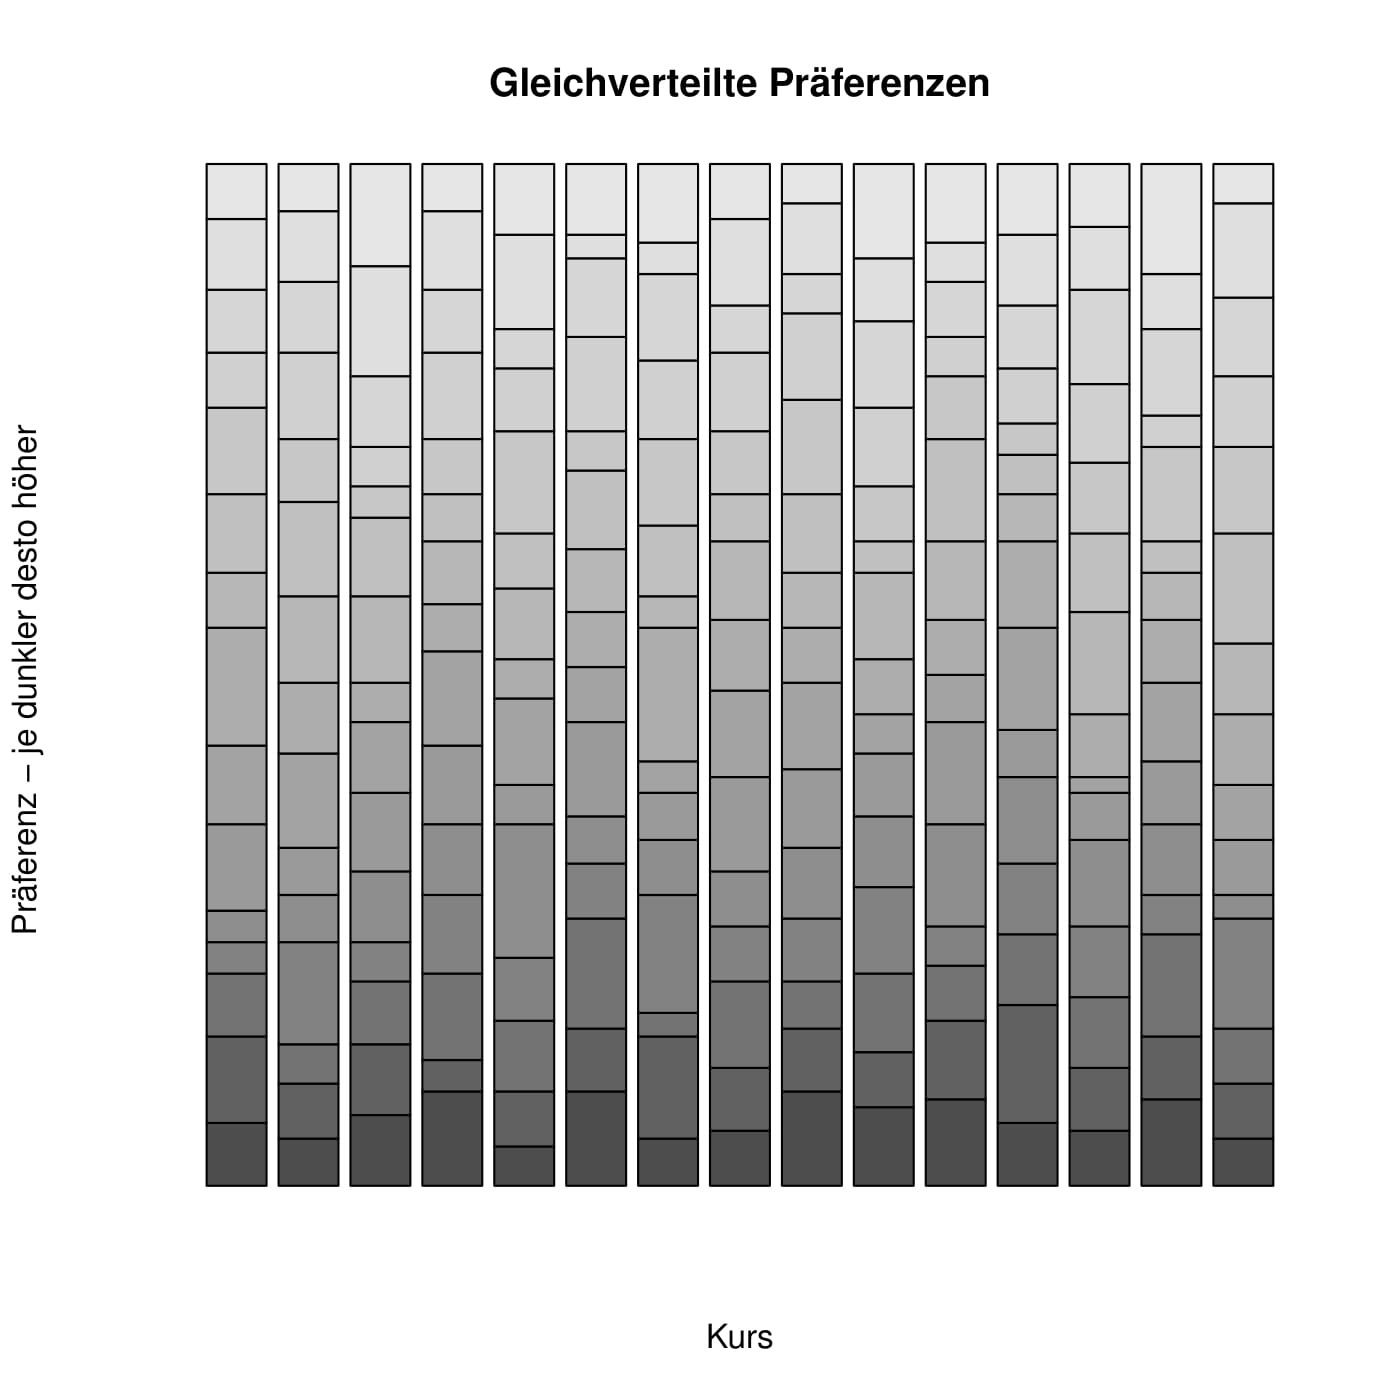
\includegraphics[width=0.7\textwidth]{./testing/images/EqualDistPreferencesDist.jpg}
				\caption{Gleichverteilte Präferenzen mit 130 Studenten auf 15 Kursen mit maximal 10 Teilnehmern pro Kurs. Die Dunkelheit stellt die Höhe der Präferenz dar}
				\label{fig:test_equal_distribution}
			\end{figure}
			Die gleichverteilte Präferenzenmatrix ist in Abbildung \ref{fig:test_equal_distribution} zu sehen.
			
			\begin{figure}
				\centering
				\begin{subfigure}{0.49\textwidth}
					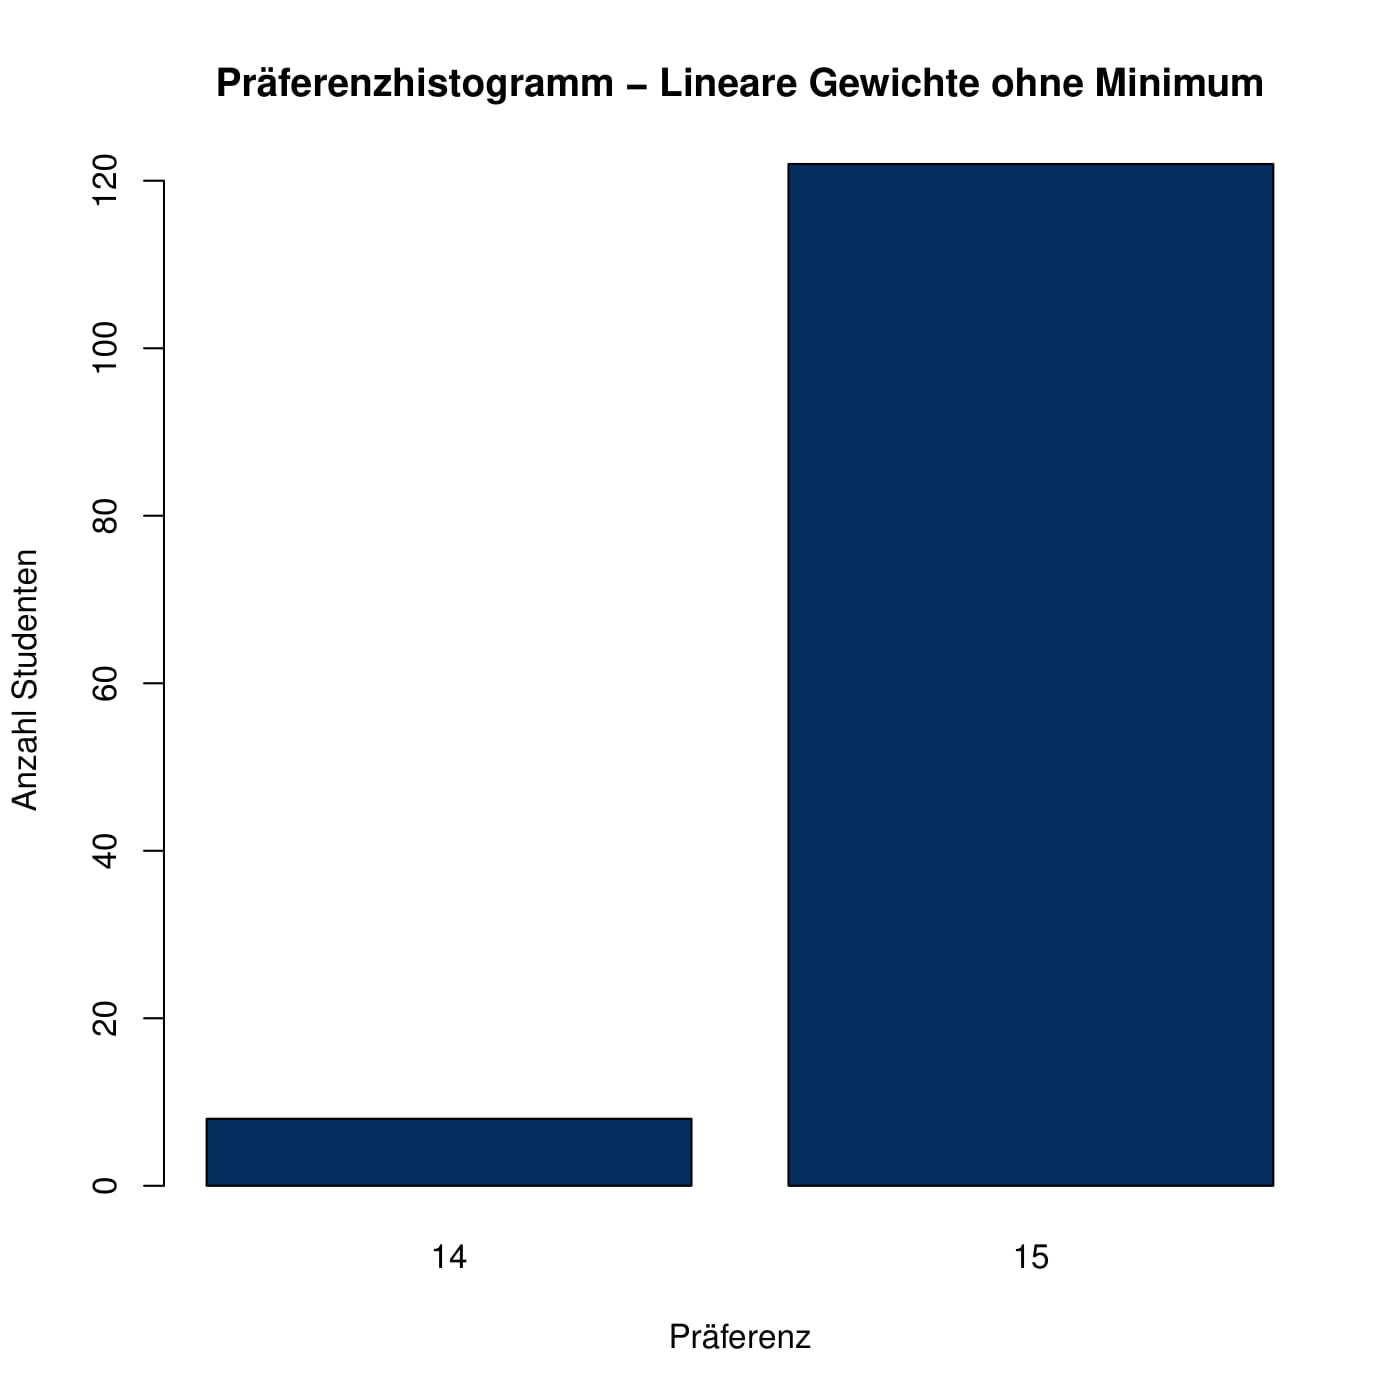
\includegraphics[width=1.0\textwidth]{./testing/images/EqualDistPreferencesHistLin.jpg}
				\end{subfigure}
				\begin{subfigure}{0.49\textwidth}
					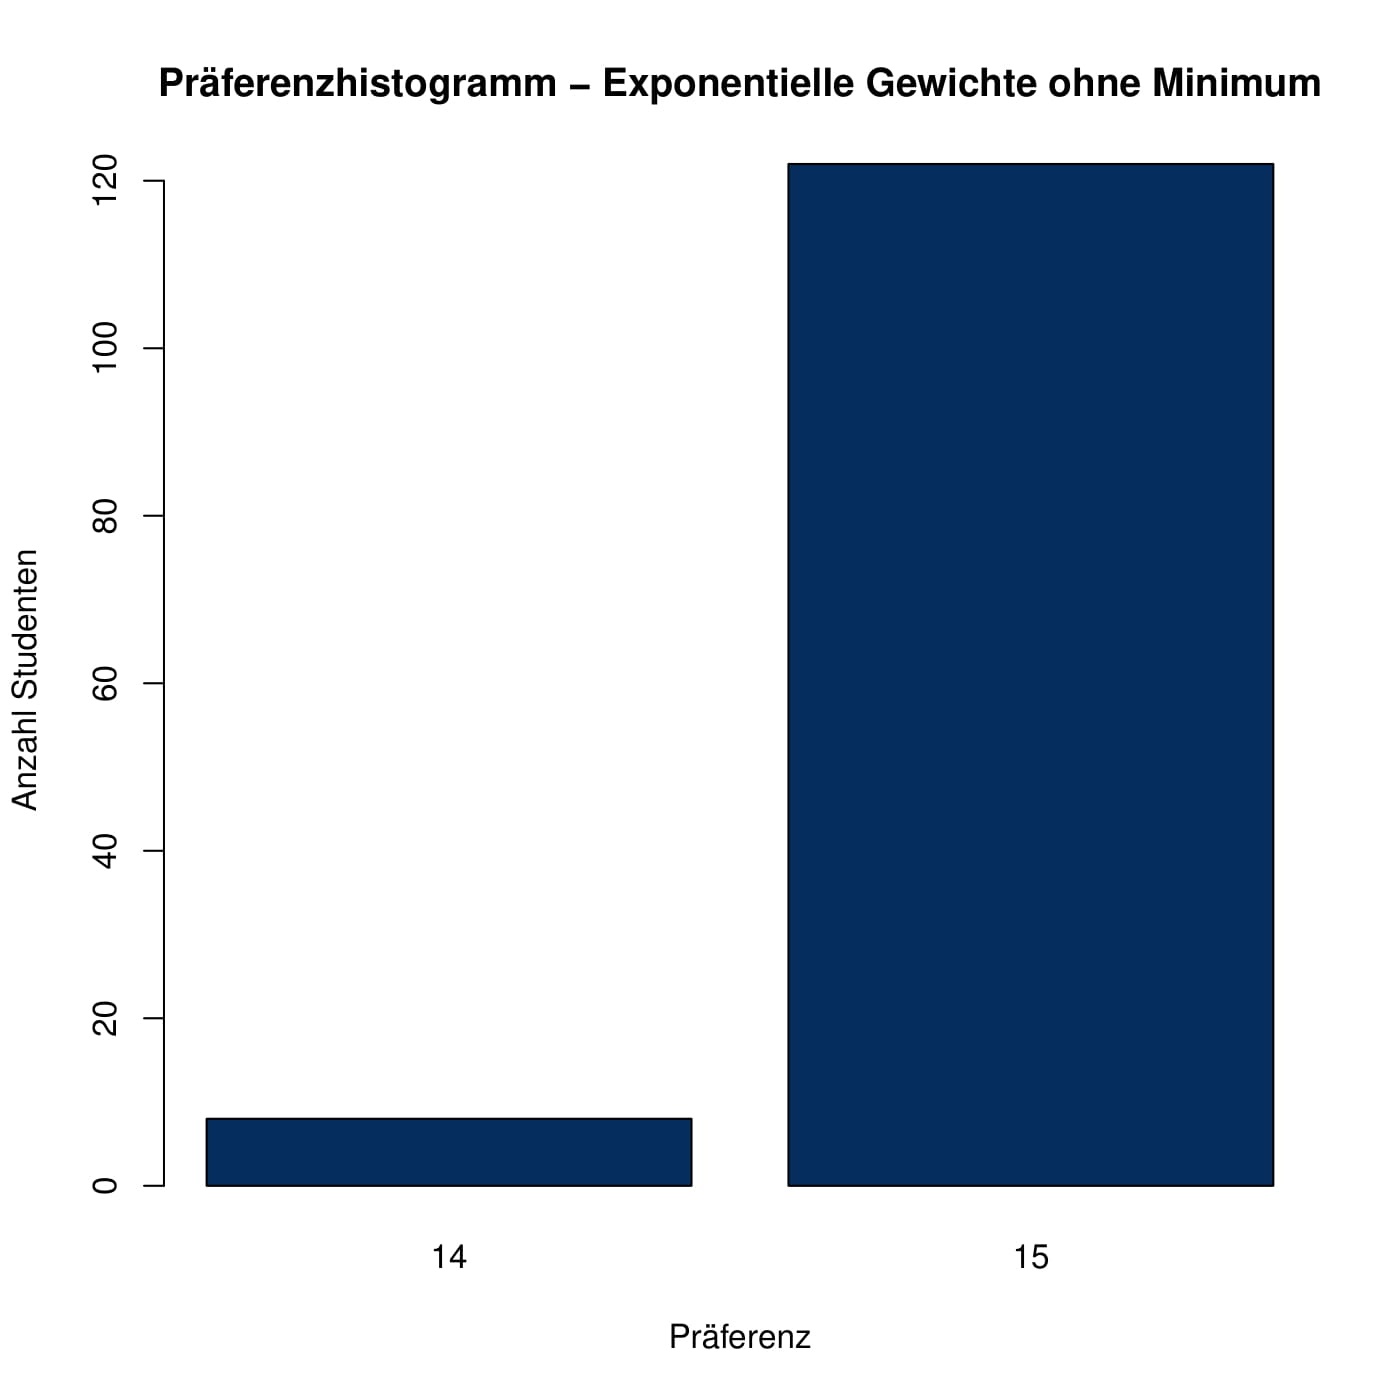
\includegraphics[width=1.0\textwidth]{./testing/images/EqualDistPreferencesHistExpo.jpg}
				\end{subfigure}
				\caption{Gegenüberstellung der Präferenzenhistogramm für lineare und exponentielle Gewichtung}
				\label{fig:test_equal_distribution_histogram}
			\end{figure}
			
			Die Verteilung ist in dem Präferenzenhistogramm in Abbildung \ref{fig:test_equal_distribution_histogram} dargestellt.\newline
			
			Wie man sieht, bekommen die meisten Studenten ihre Erstwahl, das heißt den Kurs mit Präferenz 15.
			Nur sehr wenige Studenten bekommen ihre Zweitwahl, das heißt den Kurs mit Präferenz 14.\newline
			
			Der Grund hierfür ist, dass die Präferenzen auf die Kurse gleichverteilt werden.
			Das heißt, die Wahrscheinlichkeit, dass ein beliebiger Student einen beliebigen Kurs mit beliebiger Präferenz wählt, ist immer gleich.
			Nichtsdestotrotz ist eine gewisse Varianz in der Ziehung der Präferenzen zu beobachten.
			Daher hat jeder Kurs unterschiedlich viele Studenten pro Präferenz.
			Daher kann man davon ausgehen, dass es wenige Studenten geben muss, die nur ihre Zweitwahl kriegen können.\newline
		
		\subsection{Normalverteilung}
		\label{sec:testing:normaldistribution}
		
			\begin{figure}
				\centering
				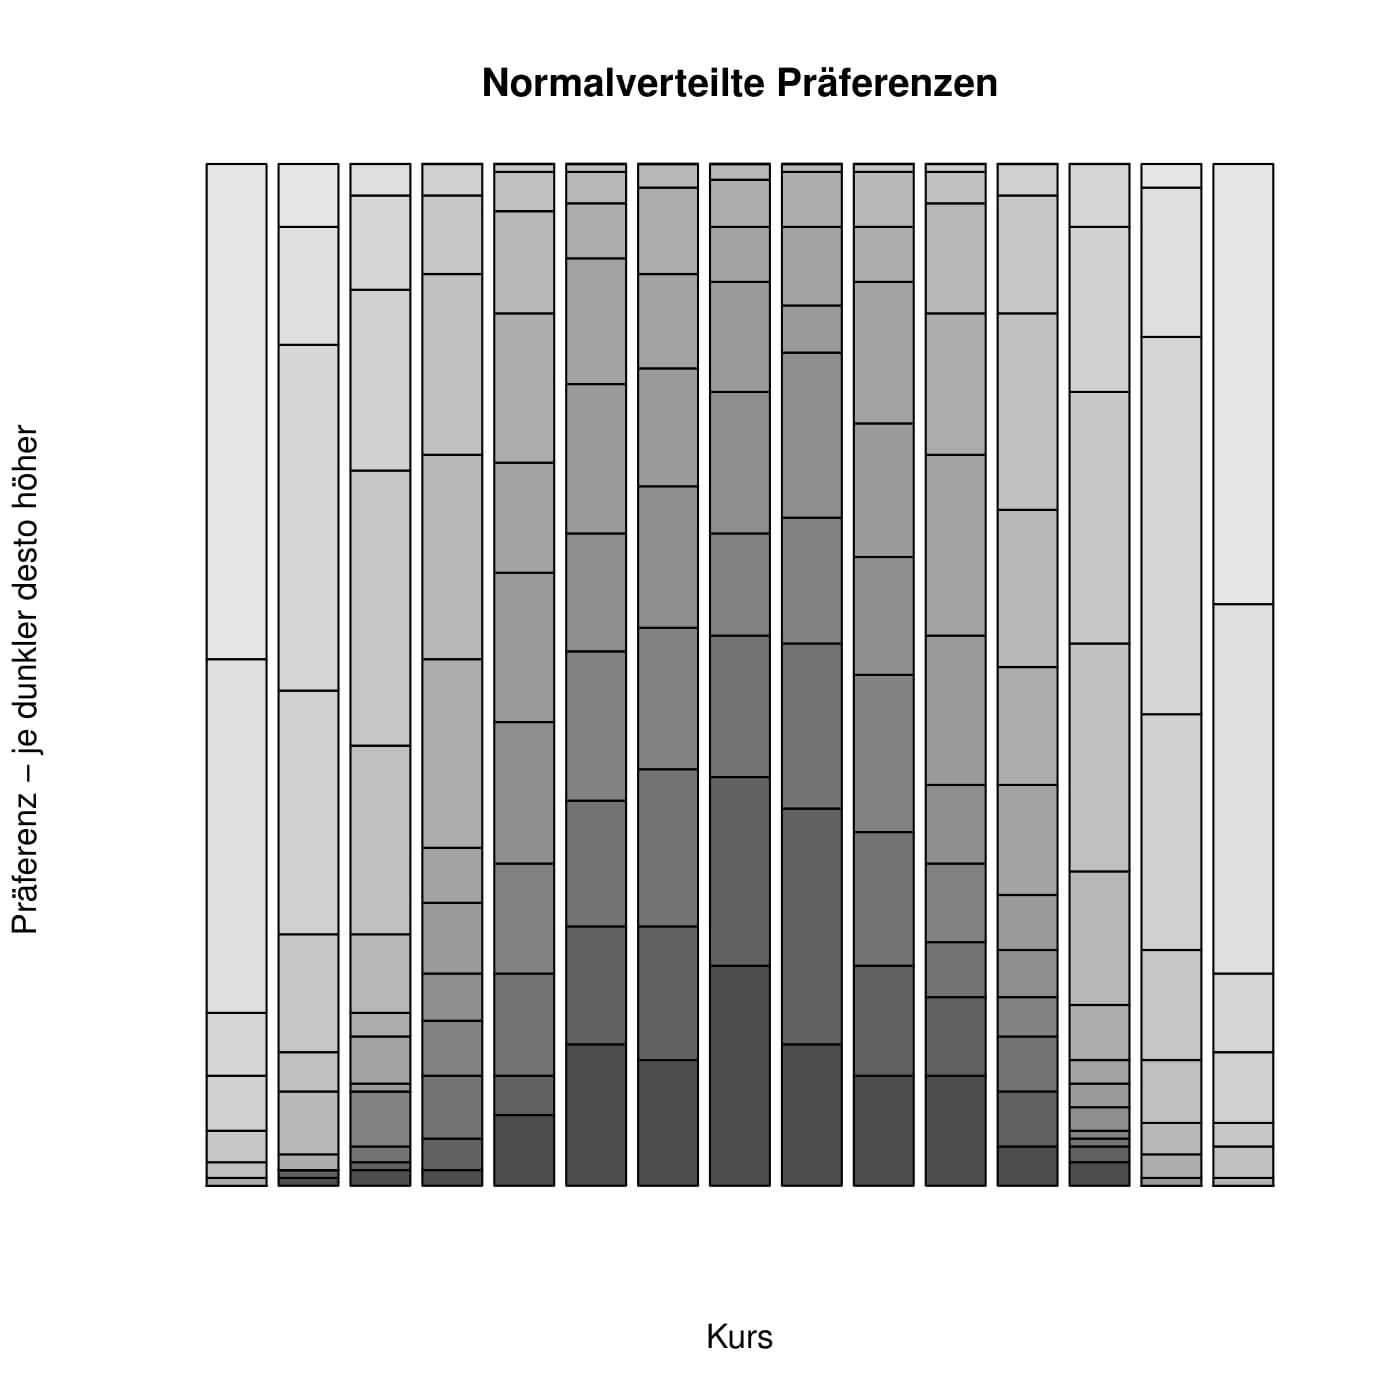
\includegraphics[width=0.7\textwidth]{./testing/images/NormalDistPreferencesDist.jpg}
				\caption{Normalverteilte Präferenzen mit 130 Studenten auf 15 Kursen mit maximal 10 Teilnehmern pro Kurs. Die Dunkelheit stellt die Höhe der Präferenz dar}
				\label{fig:test_norm_distribution}
			\end{figure}
			Die normalverteilte Präferenzenmatrix ist in Abbildung \ref{fig:test_norm_distribution} zu sehen.
			
			\begin{figure}
				\centering
				\begin{subfigure}{0.3\textwidth}
					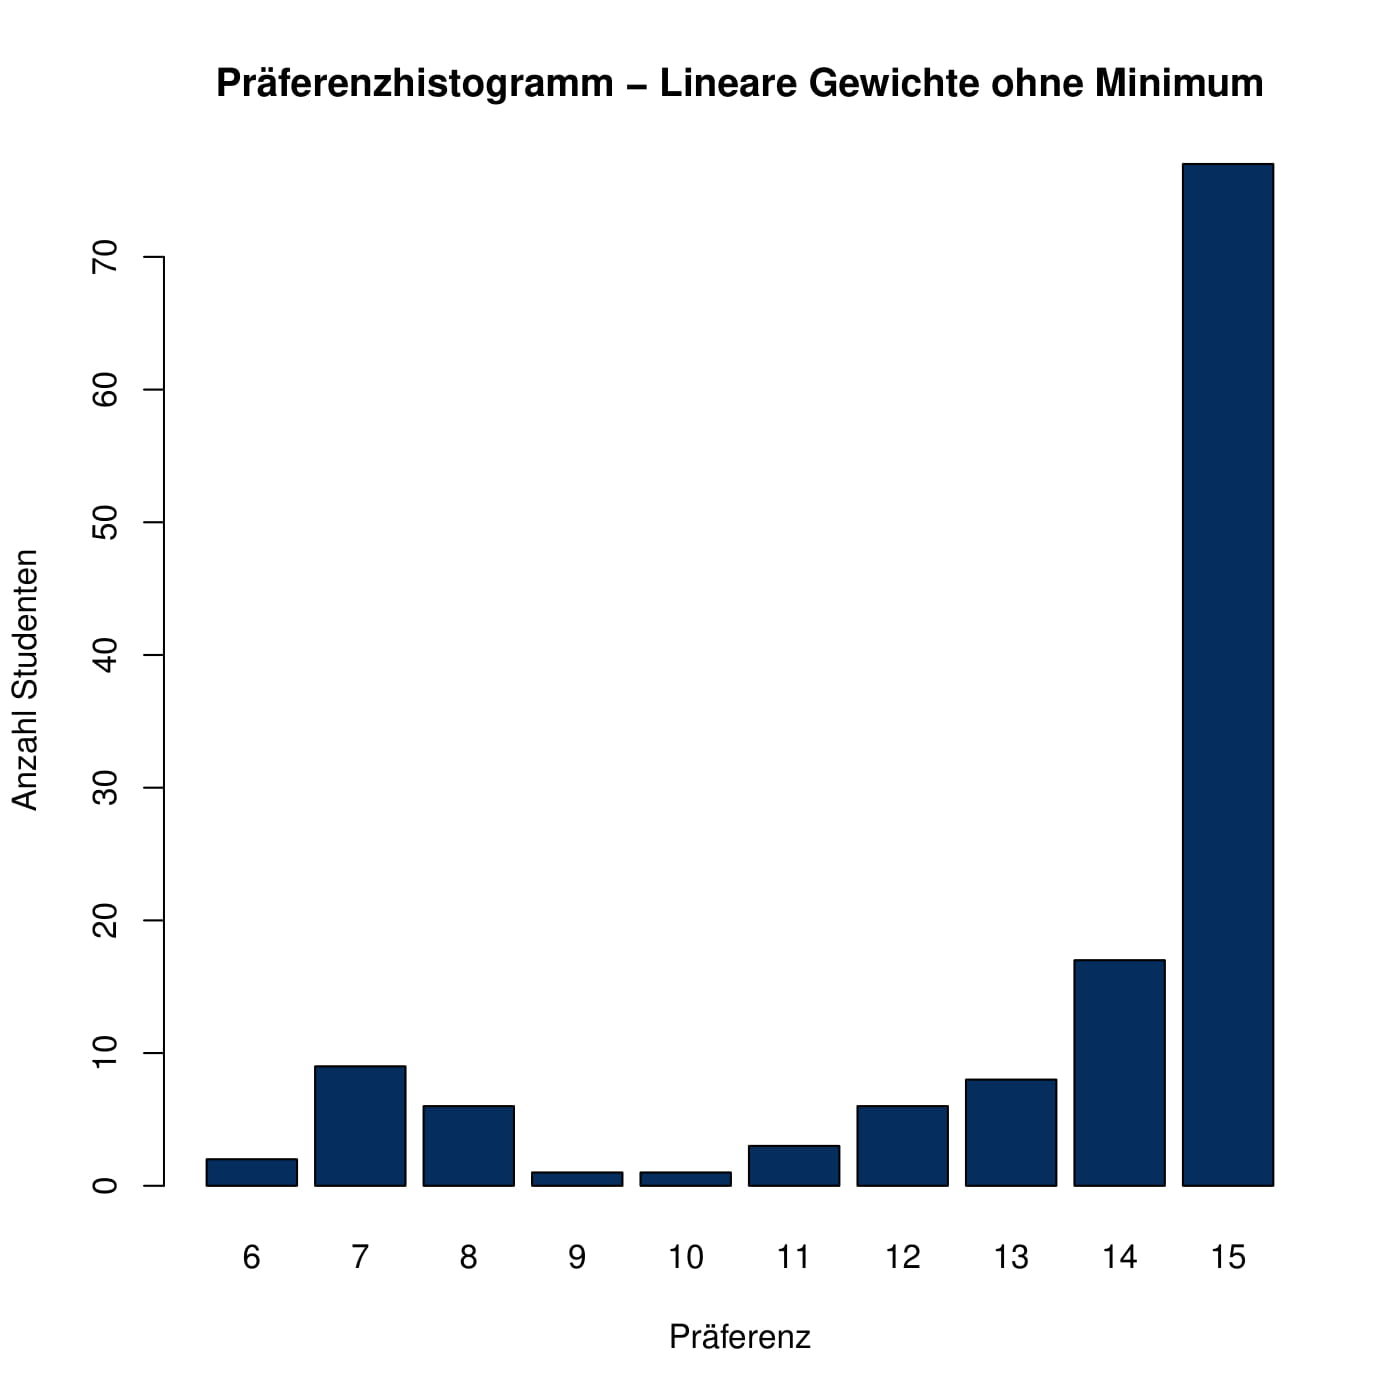
\includegraphics[width=1.0\textwidth]{./testing/images/NormalDistPreferencesHistLin.jpg}
				\end{subfigure}
				\begin{subfigure}{0.30\textwidth}
					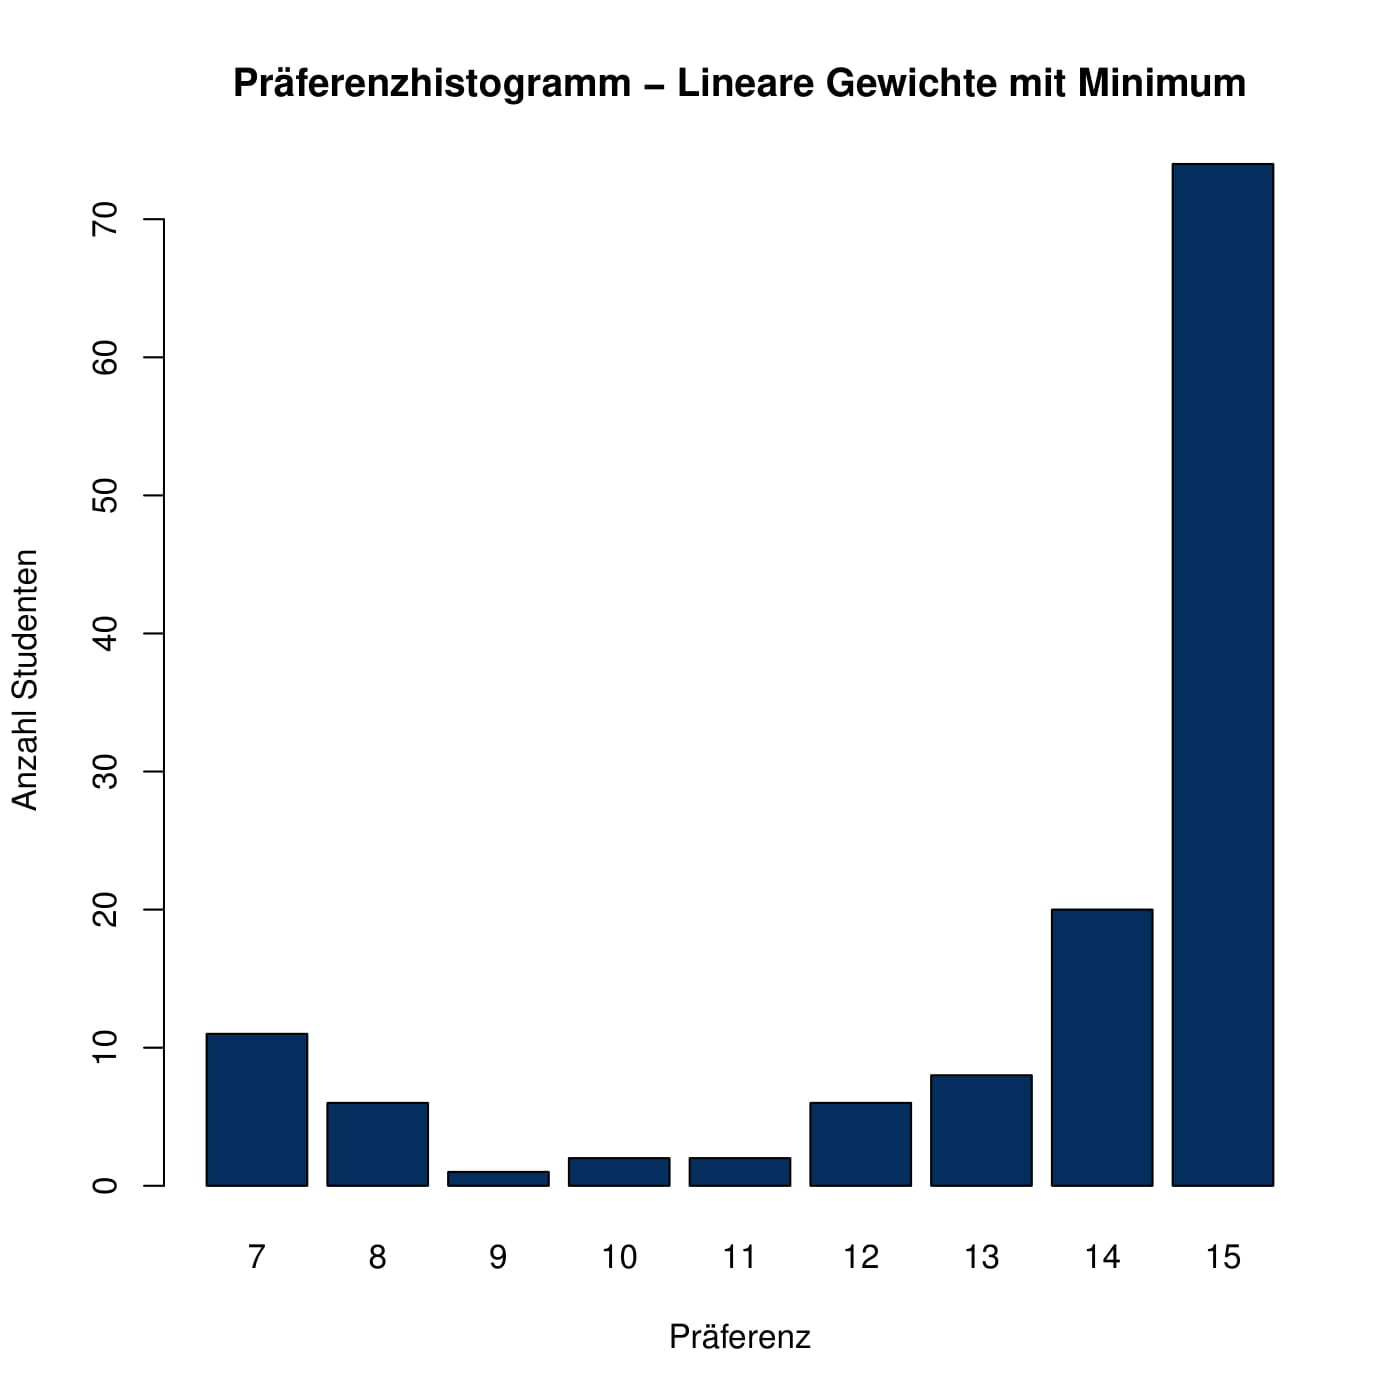
\includegraphics[width=1.0\textwidth]{./testing/images/NormalDistPreferencesHistLinMin.jpg}
				\end{subfigure}
			\begin{subfigure}{0.3\textwidth}
				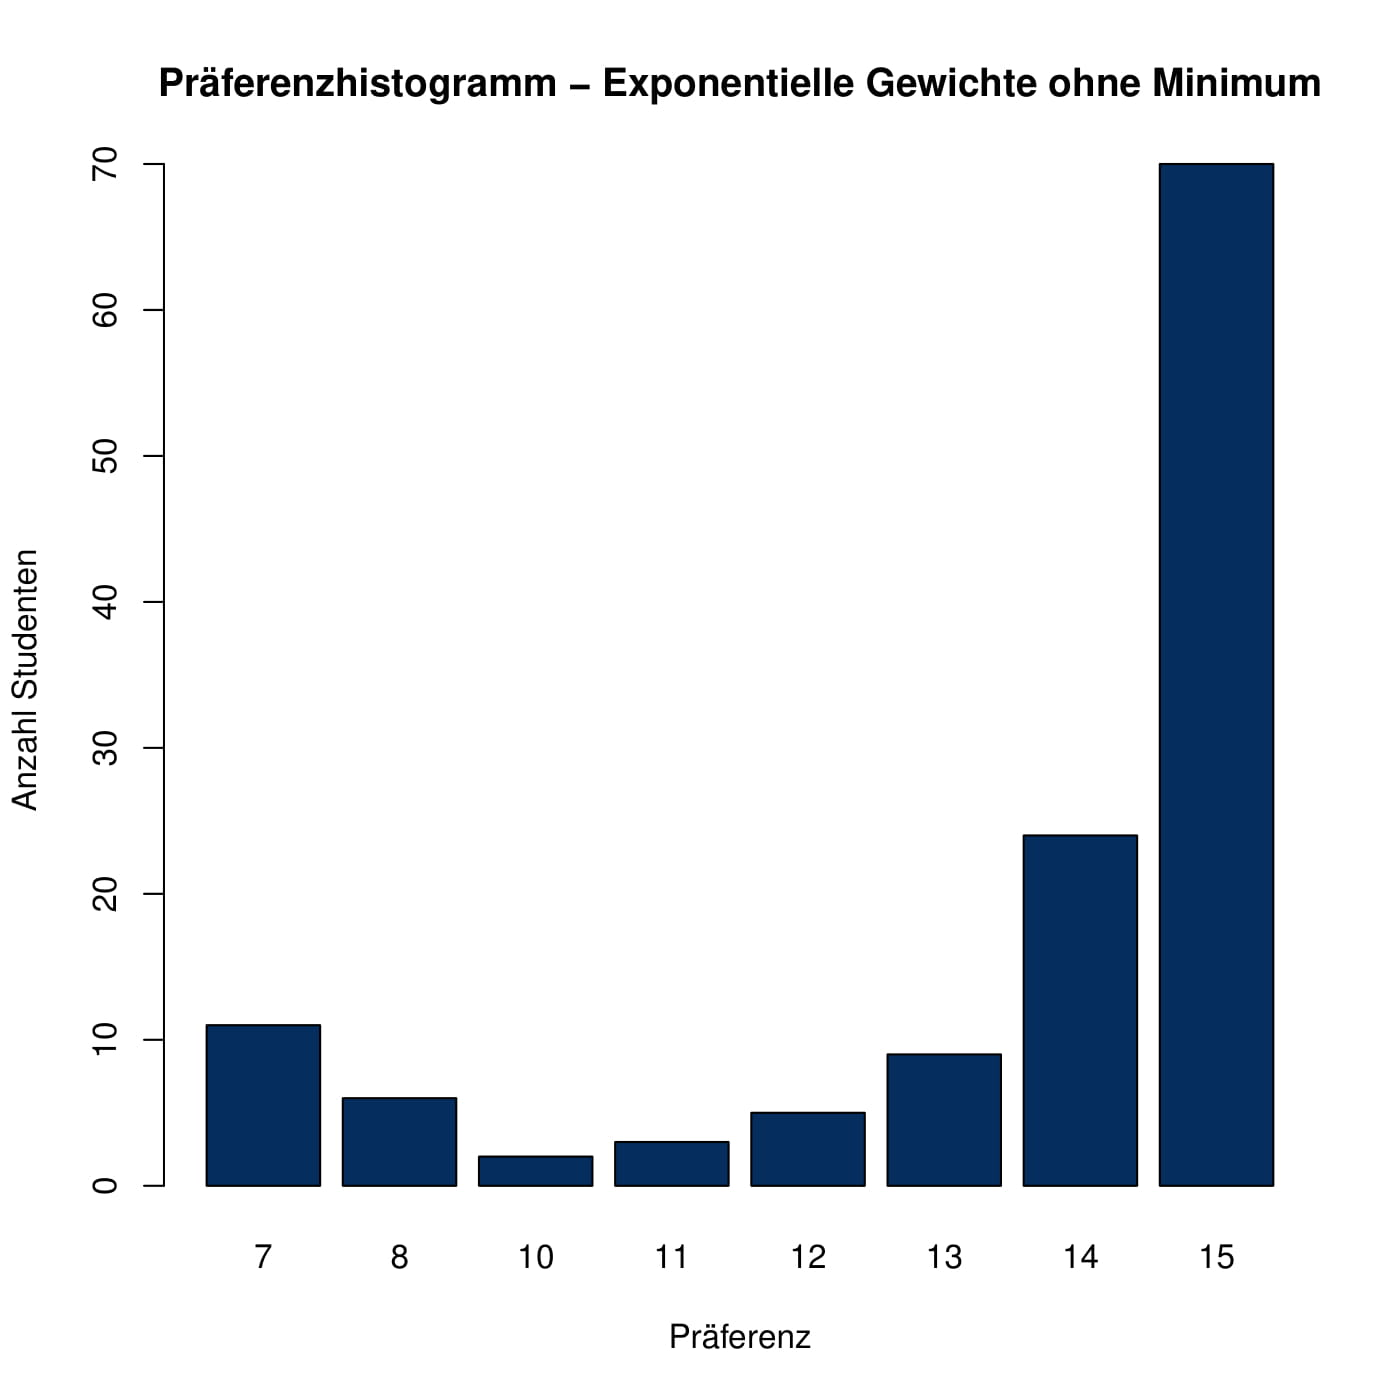
\includegraphics[width=1.0\textwidth]{./testing/images/NormalDistPreferencesHistExpo.jpg}
			\end{subfigure}
				\caption{Gegenüberstellung der Präferenzenhistogramm für lineare Gewichtung, lineare Gewichtung mit Minimum und exponentielle Gewichtung}
				\label{fig:test_norm_distribution_histogram}
			\end{figure}
		
			Die Verteilung ist in dem Präferenzenhistogramm in Abbildung \ref{fig:test_equal_distribution_histogram} dargestellt.\newline
			
			Wie man sieht, bekommen in jeder der Verteilungen mehr als die Hälfte der Studenten ihre Erstwahl.
			Um die 20 Studenten bekommen allerdings nur den Kurs mit einer Präferenz kleiner 11.\newline
			
			Gut zu sehen ist, dass die Variante \glqq Lineare Gewichte ohne Minimum\grqq~sich von \glqq Lineare Gewichte mit Minimum\grqq~unterscheidet.
			Die erste Variante hat die minimale Präferenz 6, doch durch das Erzwingen eines festen Minimums verbessert sich diese auf 7.
			Nach den Anforderungen ist dies so wünschenswert.
			Zuletzt ist in der Variante \glqq Exponentielle Gewichte ohne Minimum\grqq~zu sehen, dass weniger Studenten ihre Erstwahl erhalten, dafür aber mehr Studenten die Präferenz 10 oder höher bekommen.\newline
			
		\subsection{Realdaten}
		
			Letztlich stellte uns der Lehrstuhl, der das Empiriepraktikum leitet, die Daten aus dem Wintersemester 2017/2018 zur Verfügung, um den neuen Algorithmus mit dem alten zu vergleichen.\newline
			
			\begin{figure}
				\centering
				\begin{tabular}{l|l|l}
					& Alter Algorithmus & Neuer Algorithmus \\
					\hline
					Mittelwert & 14.2 & 14.4 \\
					Varianz & 1,8 & 0,75 \\
					Minimale Präferenz & 7 & 12 \\
				\end{tabular}
				\caption{Vergleich des alten Algorithmus mit dem neuen Algorithmus}
				\label{tab:old_versus_new_algorithm}
			\end{figure}
		
			Wie in Abbildung \ref{tab:old_versus_new_algorithm} zu sehen ist, verbessert sich der Mittelwert, die Varianz und minimale Präferenz im Gegensatz zur vorigen Variante.\newline
			
			Dadurch zeigt sich, dass der neue Algorithmus zu einem besseren Ergebnis führt.
			In Folge dessen ist der neue Verteilungsalgorithmus besser als der alte Algorithmus und erfüllt somit das Akzeptanzkriterium.
			
		\subsection{Ergebnisse des Algorithmus}
			
			Wie in dem Abschnitt \ref{sec:testing:normaldistribution} bereits erklärt, führen die Varianten des Algorithmus teilweise zu unterschiedlichen Ergebnissen.
			Wie in den Anforderungen beschrieben, soll der Administrator die Wahl haben, welche dieser Verteilungen er nutzen möchte.
			Daher wurden mehrmals Verteilungen generiert und sicher gestellt, dass die verschiedenen Verteilungen auch tatsächlich so eingetragen werden.
			Da dies sehr aufwendig ist, wurde nur verifiziert, dass die minimale Präferenz auch so im Backend vorzufinden ist.\newline

			Gleichzeitig wurde verifiziert, dass ein Bestätigen der Verteilung eine E-Mail-Benachrichtigung erfolgt.
			Dafür wurde ein Mailserver genutzt, der alle E-Mails erhält.
			Nach den Anforderungen sollten hierbei drei Typen von Mails verschickt werden.
			Wer welche Mail erhält, hängt von der Rolle des Nutzers ab.
			Studenten erhalten eine E-Mail mit Informationen, welchen Kurs sie zugeteilt bekommen haben.
			Dozenten erhalten eine E-Mail mit Informationen, welche Studenten in ihren Kursen sind.
			Administratoren erhalten eine E-Mail mit Informationen, welche Studenten welchen Kurs bekommen haben.\newline
			Für die Verifikation wurde jeweils eine E-Mail der Rolle gewählt und die Richtigkeit der Information überprüft.\newline
			
			
		
		
		
		
		
		
		
		
		
		
		
		
		
		
		
		
		
		
		
		
		
		
		
		
		
